% Bulk-boundary anomaly inflow schematic (Ch 8)
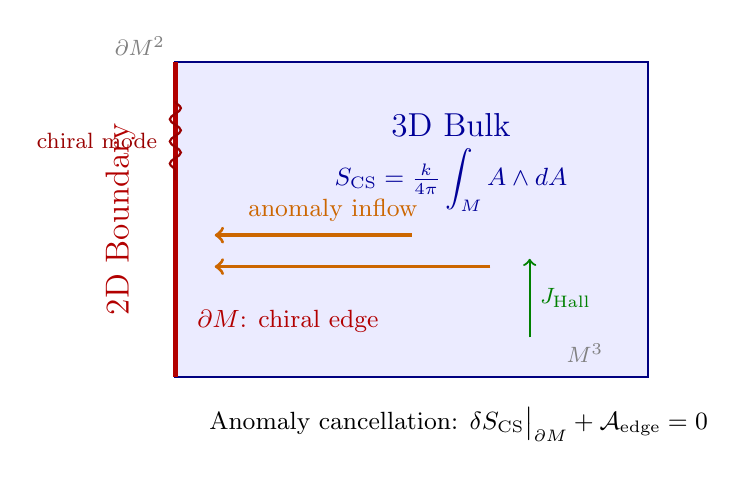
\begin{tikzpicture}[scale=1.0, thick]

  % 3D Bulk region (drawn as a shaded rectangle)
  \fill[blue!8] (0, 0) rectangle (6, 4);
  \draw[blue!50!black, thick] (0, 0) rectangle (6, 4);

  % Boundary (left edge, highlighted)
  \draw[red!70!black, ultra thick] (0, 0) -- (0, 4);

  % Bulk label
  \node[blue!60!black, font=\large] at (3.5, 3.2) {3D Bulk};
  \node[blue!60!black, font=\small] at (3.5, 2.5) {$S_{\mathrm{CS}} = \frac{k}{4\pi}\displaystyle\int_M A \wedge dA$};

  % Boundary label
  \node[red!70!black, font=\large, rotate=90] at (-0.7, 2.0) {2D Boundary};
  \node[red!70!black, font=\small, anchor=west] at (0.15, 0.7) {$\partial M$: chiral edge};

  % Anomaly inflow arrows
  \draw[->, very thick, orange!80!black] (3.0, 1.8) -- (0.5, 1.8);
  \draw[->, very thick, orange!80!black] (4.0, 1.4) -- (0.5, 1.4);
  \node[orange!80!black, font=\small, above] at (2.0, 1.85) {anomaly inflow};

  % Hall current arrow (bulk)
  \draw[->, thick, green!50!black] (4.5, 0.5) -- (4.5, 1.5);
  \node[green!50!black, font=\footnotesize, right] at (4.5, 1.0) {$J_{\mathrm{Hall}}$};

  % Edge mode (wavy line along boundary)
  \draw[red!60!black, decorate, decoration={snake, amplitude=2pt, segment length=8pt}]
    (0, 3.5) -- (0, 2.5);
  \node[red!60!black, font=\footnotesize, left] at (-0.1, 3.0) {chiral mode};

  % Key equation
  \node[font=\small, anchor=west] at (0.3, -0.6)
    {Anomaly cancellation: $\delta S_{\mathrm{CS}}\big|_{\partial M} + \mathcal{A}_{\mathrm{edge}} = 0$};

  % M label with dimension
  \node[font=\footnotesize, gray] at (5.2, 0.3) {$M^3$};
  \node[font=\footnotesize, gray, left] at (0, 4.2) {$\partial M^2$};
\end{tikzpicture}
